\section{Simulation} 

\begin{frame}{Simulation Study I}

    Data generation:
    \begin{itemize}
      \item Observations: $100$ units on a $10\times 10$ grid (adjacent if sharing a boundary).
      \item Spatial effect: $\phi_i$ simulated with $\tau=1$, $\rho=0.9$.
      \item Covariates: $x_i\in\mathbb{R}^2$ i.i.d.\ Gaussian.
      \item Fixed cluster labels and cluster specific regression coefficients $\beta_k$.
      \item Outcome: $y_i=\phi_i+x_i^\top\beta_k+\varepsilon_i$, \;\; $\varepsilon_i \stackrel{\text{iid}}{\sim} \mathcal{N}(0,1)$.
      \item Experiments: $K_0=4$ and $K_0=7$.
    \end{itemize}

\end{frame}

\begin{frame}{Simulation Study II}
    \centering
    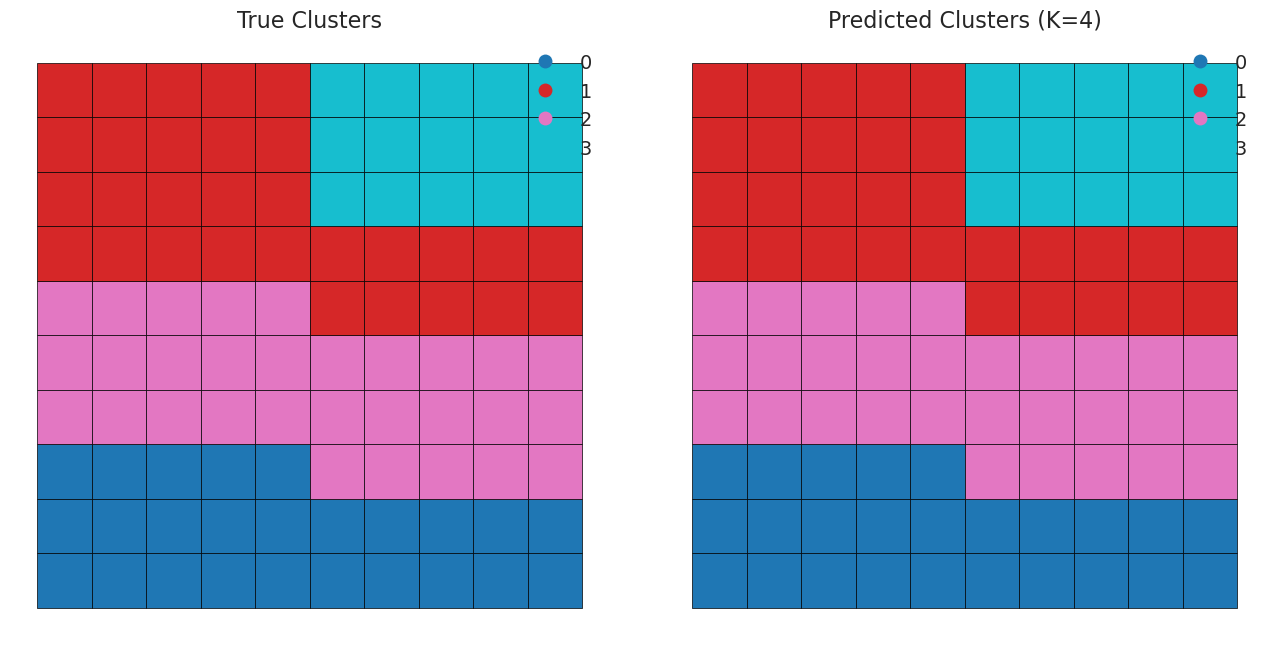
\includegraphics[width=0.7\textwidth]{pictures_second_presentation/k4-simulated.png} 

    
    \small
    Comparison between true cluster label and predicted cluster label for the model with $K_0=4$
\end{frame}

\begin{frame}{Simulation Study III}
    \centering
    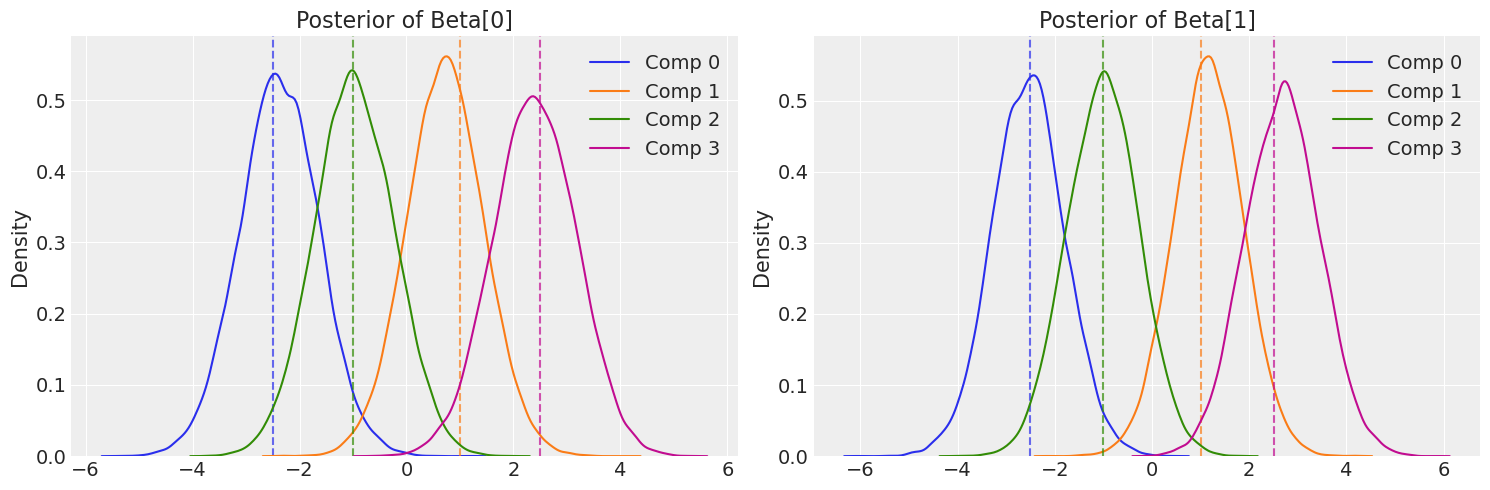
\includegraphics[width=\textwidth]{pictures_second_presentation/betaposterior-truevalue.png}

    \small
    Posterior density of the cluster-specific regression coefficients $\beta$ and their true value for the $K_0 = 4$ configuration.
\end{frame}


\begin{frame}{Simulation Study IV}
    \centering
    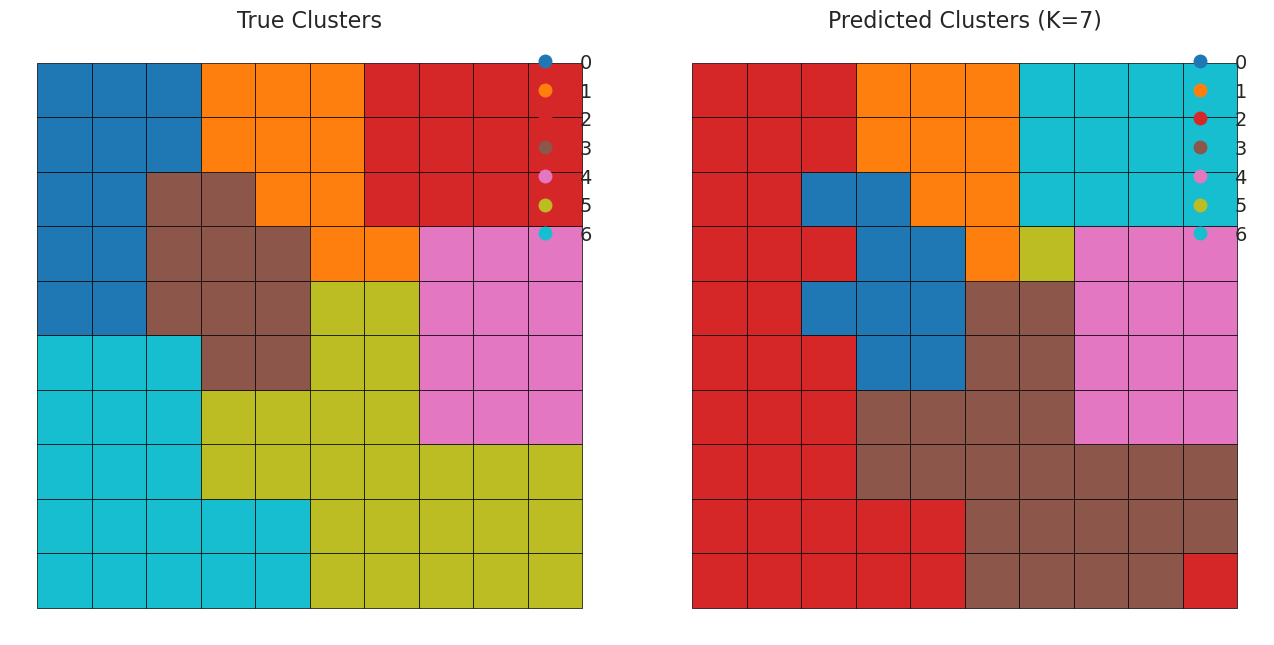
\includegraphics[width=0.7\textwidth]{pictures_second_presentation/k7-simulated.png}

    \small
    Comparison between true cluster label and predicted cluster label for the model with $K_0=7$
\end{frame}